\documentclass{beamer}

\usepackage[utf8]{inputenc}
\usepackage{default}
\usepackage{tikz}
\usetikzlibrary{shapes,decorations}
\usepackage{smartdiagram}
\usepackage{xstring}
%\smartdiagramset{set color list={
 % green!40!lime!80!black,
  %cyan!80!blue,
  %orange!50!red,
 %},
 %sequence item border color=gray!30!black,
%}
\begin{document}

\title{NGS Quality Control}
\subtitle{Projektmanagement im Softwarebereich - SeqAn 2013}
\author{Daniel Kersting \and Antje Oldenburg}
\date{Berlin, 24. April, 2013}
\subject{Informatik}


\frame{\titlepage}

\begin{frame}
  \frametitle{Background NGS Quality Control}
  \framesubtitle{}
   Vorbilder: FastQC FastX, PrinSeq\pause
  \begin{center}
  \includegraphics<2>[width=0.65\textwidth, angle=0]{fastqc.png}\pause
  \includegraphics<3>[width=0.65\textwidth, angle=0]{FastX.png}\pause
  \includegraphics<4>[width=0.65\textwidth, angle=0]{PrinSeq.png}
  \end{center}
\end{frame}

\begin{frame}

%\begin{center}
 %\smartdiagram[circular diagram]{Initiation,Planning,Execution,Closure}
%\end{center}

  \frametitle{Functional Overview}
  \begin{center}
  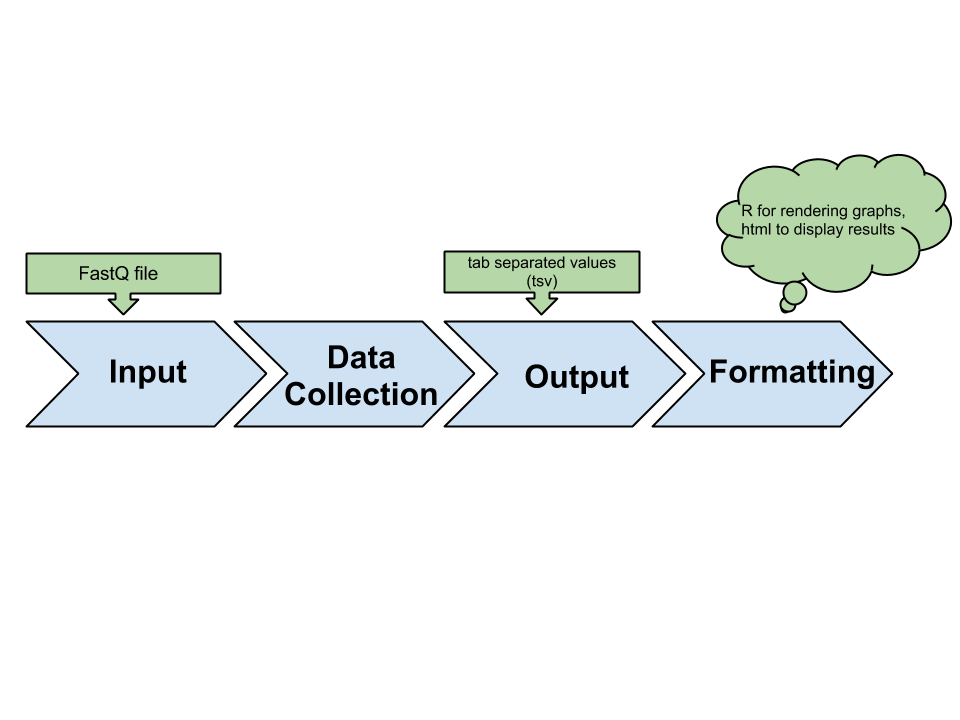
\includegraphics[width=1\textwidth, angle=0]{Flussdiagramm.png}
  \end{center}
  %\begin{description}
   %\item[Input] fastq file
   %\item[Data collection] 
   %\item[Output] tab separated values (tsv)
   %\item[Formatting] R for rendering graphs, html to display results 
  %\end{description}

\end{frame}



\begin{frame}
 \frametitle{ Statistical Information we plan to show}
 \framesubtitle{and how we collect the data for it}

 We grouped our quality metrics into groups, depending on 
 wether it describes data 

 \begin{enumerate}
  \item about the whole file
  \item about all reads
  \item all positions in all reads 
 \end{enumerate}

This reflects where we collect the data:
\begin{itemize}
\item open seqan::SequenceStream
  \begin{itemize}
  \item read Record
    \begin{itemize}
    \item read nucleotide and quality and update data object
    \end{itemize}
  \end{itemize}
\end{itemize}
 
\end{frame}



\begin{frame}
 \frametitle{ Simple statistics about all positions in all reads }
 \framesubtitle{and how we collect the data for it}

Our data object holds:

 \begin{itemize}
  \item a 2-dimensional counter for score per position 
  \item a 2-dimensional counter for Dna5 element per position 
 \end{itemize}

This will enable us to collect the following data:

\begin{itemize}
 \item basic quality distribution data: median, mean, quantiles (10,25,75,90)
 \item distribution of [A,C,G,T]
 \item GC percent content
 \item N Content
\end{itemize}

\end{frame}


\begin{frame}
 \frametitle{ Statistics about about all reads}
 \framesubtitle{and how we collect the data for it}

Our data object holds:

 \begin{itemize}
  \item a 2-dimensional counter for score per position 
  \item counter for encountered sequence lengths 
 \end{itemize}

This will enable us to collect the following data:
  \begin{itemize}
    \item mean qualities distribution
    \item sequence length distribution
  \end{itemize}
\end{frame}



\begin{frame}
 \frametitle{ Statistics about the whole file}
 \framesubtitle{and how we collect the data for it}

Our data object holds:

 \begin{itemize}
  \item all program arguments, explicitly set and not 
  \item a 2-dimensional counter for score per position 
  \item a 2-dimensional counter for Dna5 element per position 
  \item a counter for the number of records encountered
 \end{itemize}

This will enable us to collect the following data:
\begin{itemize}
 \item   input filename and format
 \item which scoring system was used
 \item   total number of sequences
 \item   overall quality score average of all bases in all sequences
 \item   overall GC percent
 \item   overall N percent
\end{itemize}
\end{frame}


\begin{frame}
 \frametitle{ K-mer content statistics}
 \framesubtitle{k-mer distribution}
\begin{description}
 \item[Goal] Find plentiful k-mer  
 \item[Problem] memory and time contraints
 \item[Strategy] found and count 
    \begin{enumerate}
      \item create k-mer index
      \item count each k-mer for each position
    \end{enumerate}
 \item[Implementation]\hfill\\
 %\begin{itemize}
% \hspace*{-5cm} 
 %\item 
 \vspace*{.5cm}
 \hspace*{-2cm}\footnotesize{\texttt{String<Dna5> genome}}\\
  %\item 
  \hspace*{-2cm}\footnotesize{\texttt{Index<String<Dna5>, IndexEsa<> > esaIndex(genome)}}\\
  %\item 
  \hspace*{-2cm}\footnotesize{\texttt{Finder<Index<String<Dna5>, IndexEsa<> > > esaFinder(esaIndex)}} \\
  %\item 
  \hspace*{-2cm}\footnotesize{\texttt{find(esaFinder)}} for each \small{\texttt{k-mer}}\\
  %\item 
  \hspace*{-2cm}\footnotesize{save in Matrix (position,all k-mer,count)}
  
 %\end{itemize}
\end{description}
\end{frame}
\begin{frame}
 \frametitle{ K-mer content statistics}
 \framesubtitle{k-mer distribution}
   \begin{center}
  \includegraphics<1>[width=0.65\textwidth, angle=0]{kmer2.png}\pause
  \includegraphics<2>[width=0.65\textwidth, angle=0]{kmer1.png}

  \end{center}
%% describe how you'll do that

\end{frame}


\begin{frame}
 \frametitle{sequence duplication}
 \framesubtitle{and how we collect the data for it}
\begin{description}
 \item[Goal] Detect fully duplicated reads  
 \item[Problem] memory and time contraints
 \item[Strategy] for n reads contained in dataset 
    \begin{enumerate}
      \item collect the first k reads and create a suffix array
      \item starting from k, increment a counter if exact matches occur 
    \end{enumerate}
 \item[Implementation]
 \begin{itemize}
  \item \small{\texttt{<StringSet<Dna5> >}} as haystack
  \item \small{\texttt{appendValue}} to haystack k times
  \item \small{\texttt{Index}} as \small{\texttt{ IndexEsa<>}} 
  \item \small{\texttt{clear}} and \small{\texttt{find}} on \small{\texttt{IndexEsa<>}}
 \end{itemize}
 \item[Implications] If used for 200.000 reads of length 100, needed memory for this would be 20 MBytes.
\end{description}


\end{frame}




\begin{frame}
 \frametitle{Data output and formatting}
 \framesubtitle{Steps to create a visual summary}
\begin{enumerate}
 \item output tsv file with tabular data from our data 
 \item secondary app: script that does
  \begin{enumerate}
   \item creates a static R script
   \item calls R script on tsv to create png's
   \item creates a static html file that displays results   
  \end{enumerate}
\end{enumerate}
 
\end{frame}


\begin{frame}
 \frametitle{NICE-TO-HAVEs}
 \framesubtitle{what we want to add if time allows}
\begin{itemize}
 \item read for data formats: fastq compressed, bam, sam, 
 \item sequence complexity statistics
 \item KNIME integration
 \item Galaxy integration
\end{itemize}

\end{frame}


\begin{frame}
 \frametitle{ Milestones }
 \begin{description}
  \item [1st week] testing and implementation of a functionally minimal version that works through all steps
  \item [2nd week] testing an implementation of all basic statistics~(A) and k-mer content~(D)
  \item [3rd week] testing and implementation of sequence duplication~(A) and output refinement~(D)
  \item [4th week] buffer for surprises, testing and implementation of \texttt{NICE-TO-HAVE} features~(A+D) 
 \end{description}
 
\end{frame}



\end{document}



   * Definition von Milestones + Einordnung in einen zeitlichen Ablaufplan? (z.B. Gant-Chart)
